\documentclass[11pt]{utalcaDoc}
\usepackage[activeacute,spanish]{babel}
\usepackage[utf8]{inputenc}
\usepackage{verbatim}
\usepackage[spanish]{babel}
%\usepackage{graphicx}
%\usepackage{latexsym}
%\usepackage{amsmath}
%\usepackage{amssymb}
%\usepackage{amsthm}
%\usepackage{anysize}
%\marginsize{2cm}{2cm}{1.7cm}{1.5cm}
\usepackage[top=2.7cm, bottom=2cm, left=1.8cm, right=1.8cm,headheight=110pt]{geometry}
\usepackage{url}
\usepackage{float}
\usepackage{amsfonts}
\usepackage{listings} % Mostrar código
%\usepackage{algorithmicx}
%\usepackage{algcompatible}
%\usepackage[noend]{algpseudocode}
%\usepackage{algorithm}
%\usepackage{algorithmic}

%\usepackage{listings}

%\usepackage{bussproofs} % pruebas lógicas

\usepackage{fancyhdr}

% aqui definimos el encabezado de las paginas pares e impares.
\lhead[Construcción de Software -- 2017-2]{Construcción de Software -- 2017-2}
%\chead[y1]{y2}
\rhead[Universidad de Talca]{Universidad de Talca}
\renewcommand{\headrulewidth}{0.5pt}



% aqui definimos el pie de pagina de las paginas pares e impares.
%\lfoot[d1]{e1}
%\cfoot[c1]{d2}
\rfoot[Victor Reyes Medina]{Victor Reyes Medina}
\renewcommand{\footrulewidth}{0.5pt}
\pagestyle{fancy} 


% Plantilla inicialmente de rapa, luego le fuí cambiando/agregando algunas cosas

\title{{\bf \Large Construcción de Software \\ 
			Prueba unidad \# 1 -- Parte II}\\ 
			{\normalsize Semestre 2017-2 -- Prof. Daniel Moreno}} 
\author{
  Victor Reyes Medina\\
  \texttt{vireyes14@alumnos.utalca.cl}
}                                               
\date{\today}                                   

\begin{document}
\renewcommand{\figurename}{Figura~}
\renewcommand{\tablename}{Tabla~}
\renewcommand{\lstlistingname}{Código~}
\renewcommand{\theenumii}{\arabic{enumii}}
\renewcommand{\labelenumii}{%
 %\theenumi.\theenumii.
  \theenumii.
}
\maketitle


\section*{a. Camino Crítico}
A continuación se presenta la tabla de actividades a realizar con su correspondiente esfuerzo:

\begin{tabular}{|c|p{9.5cm}|p{3cm} |c|}
\hline 
\textbf{Tarea} & \textbf{Descripción} & \textbf{Predecesoras} & \textbf{Esfuerzo}\\ 
\hline 
A & Crear nuevas bebidas en el sistema y persistencia de las mismas. & - & 3 días  \\ 
\hline 
B & Agregar bebidas a una cotización. & A & 2 días \\ 
\hline 
C & Crear nuevos toppings en el sistema y persistencia de los mismos. & - & 3 días  \\ 
\hline 
D & Agregar toppings a la cotización de una bebida. & C, B & 1 día  \\ 
\hline 
E & Eliminar Bebidas y Toppings del sistema. & A, C & 1 día  \\ 
\hline 
F & Editar Bebidas y Toppings guardados en el sistema. & A, C & 2 días  \\ 
\hline 
G & Agregar más de una combinación bebida-topping a la cotización & D & 1 día  \\ 
\hline 
H & Revisión del código y estandarización del mismo. & E, F, G & 2 días  \\ 
\hline 
I & Pruebas. & H & 2 días  \\ 
\hline
J & Instalación del sistema. & I & 1 día  \\ 
\hline

\end{tabular} 

Lo cual resulta en el siguiente diagrama de flechas con su respectiva ruta crítica destacada en color rojo:

\begin{figure}[H]
\includegraphics[scale=0.45]{arrows.png}
\end{figure}

\section*{b. Diseño del Sistema}

\subsection*{Casos de Uso}

A modo general se ha creado el siguiente diagrama de casos de uso que incluye las funcionalidades que tiene y tendrá en un futuro el sistema.

\begin{figure}[H]
\includegraphics[scale=0.5]{UC.jpg}
\end{figure}


\subsection*{Diagrama de Clases}

El diagrama de las clases diseñado para la implementación es el siguiente (también disponible en \url{https://goo.gl/mj18dc}):
\begin{figure}[H]
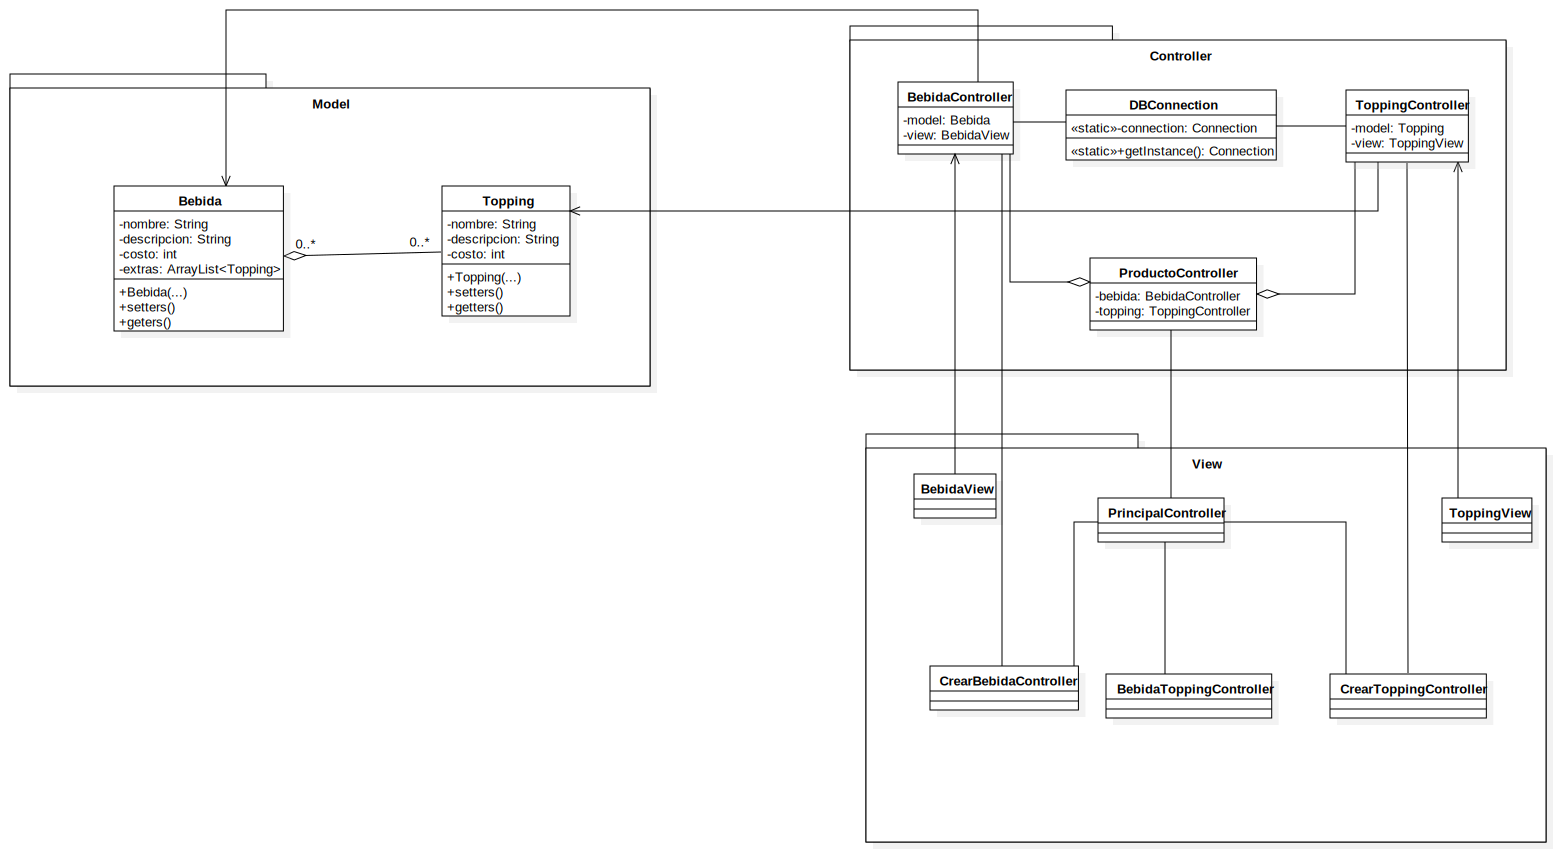
\includegraphics[scale=0.3]{CLASS.jpg}
\end{figure} 

\subsection*{Entidad Relación}

La base de datos implementada cuenta con solo dos entidades independientes:
\begin{figure}[H]
\includegraphics[scale=0.6]{ER.png}
\end{figure}

Dicha base de datos ha sido implementada usando \texttt{SQLite3}.

\section*{c. Construcción de la aplicación}

En la carpeta entregada, dentro de  \texttt{src} podrá encontrar en código fuente. En la carpeta \texttt{ejecutable} podrá encontrar el archivo \texttt{McDolan.jar} que ejecuta el programa además de las carpetas \texttt{lib} y \texttt{bd} las cuales son necesarias para la ejecución del sistema. La primera de ellas contiene la librería \texttt{SQLite3} que es usada para la conexión con la base de datos del sistema. La segunda carpeta contiene el archivo \texttt{McDolan.db} que corresponde a la base de datos, además del archivo \texttt{script.sql} usado para su creación.

Cabe destacar que la aplicación no cumple con la totalidad de las funcionalidades propuestas en el apartado (\textbf{b.}). Las funcionalidades actualmente implementadas son las siguientes:

Se define ``producto'' como la combinación de una bebida y un topping (o sin un topping). Actualmente la aplicación \textit{puede} manejar múltiples toppings por producto, pero esa funcionalidad no está implementada a nivel gráfico.

\begin{itemize}
\item Creación de bebidas en el sistema y su registro en la base de datos.
\item Creación de toppings en el sistema y su registro en la base de datos.
\item Agregación de un producto a la cotización. Es decir, seleccionar una bebida y solamente un topping.
\item Agregación múltiples productos a la cotización.
\item Visualización del costo total de la cotización, sumando por cada producto el precio base de su bebida mas el precio de \textit{cada uno} de los toppings agregados.
\end{itemize}

\section*{d. Patrones de Diseño}

Se han usado dos patrones de diseño simples MVC y Singleton. El primero a sido usado para mantener una clara separación entre lo que corresponde al modelo de datos, las interfaces de usuario y los controladores del modelo de datos.

El segundo patrón implementado corresponde al usado para mantener solo una instancia de la conexión con la base de datos y así evitar posibles retrasos debido a la constante utilización de ella y el hecho de que crear una nueva instancia puede llevar a posibles retrasos innecesarios de la aplicación.

\end{document}

